\documentclass[12pt]{article}
\usepackage{notes-common}
\usepackage{graphicx}
\geometry{margin=0.35in}
\AtBeginDocument{\fontsize{14}{17}\selectfont}

% Magnetic force and torque on current-carrying wires/loops (Knight
% 29.8-29.9). Sec.1-2 built around Example 29.13 (magnetic levitation): a
% straight copper wire floats in a horizontal field when the magnetic force
% on it exactly balances gravity. Sec.3-4 build the torque-on-a-loop result
% (Eq 29.28/29.29) and work an original numerical example (not from the
% book) using Figure 29.48's square loop.
% See magnetic-force-torque-notes-key.tex for the filled-in version.
\newcommand{\eqline}[2][-0.5mm]{%
  \par\vspace{1mm}\noindent #2\par\vspace{#1}%
  \noindent\textcolor{rulehue}{\rule{\linewidth}{0.5pt}}\par\vspace{4mm}%
}

\begin{document}

\noteshead{Magnetic Force and Torque on Current-Carrying Wires}{}

\goal{
\begin{itemize}[itemsep=5pt,parsep=2pt,topsep=2pt]
\item See where the force on a current-carrying wire, $F=IlB\sin\alpha$,
comes from --- it's just $q\vec v\times\vec B$ summed over every moving
charge in the wire.
\item Use the right-hand rule both ways: given $I$ and $\vec B$, find
$\vec F$; and given the $\vec F$ you need, find the current direction
that produces it.
\item Work a full numerical example end to end: find the current that
lets a wire ``float'' against gravity in a magnetic field (Example
29.13).
\item See why a current \emph{loop} in a field feels a net torque even
though it feels no net force, and derive $\tau=mB\sin\theta$.
\item Work a full numerical example applying $\tau=mB\sin\theta$ to a
multi-turn coil.
\end{itemize}}

%============================================================
\nsec{Where the force on a wire comes from}

A current is moving charge. A short segment of wire, length $\Delta x$,
carrying charge $\Delta q$ with drift velocity $\vec v_{\text d}$, feels
the same magnetic force as any moving charge: $F=\Delta q\,v_{\text
d}B$. The charge crosses the segment in a time $\Delta t=\Delta
x/v_{\text d}$, so $\Delta q = $ \bl[3cm]  (in terms of $I$ and
$\Delta t$). Substituting:

\[
F = \Delta q\, v_{\text d} B = \bl[6cm]
\]

Adding up every such segment over the full length $l$ of wire (when
the wire is perpendicular to $\vec B$) gives $F=IlB$. More generally,
for a wire at angle $\alpha$ to the field:

\result[1.8cm]{$\vec F_{\text{wire}} = $}

\checkpoint{The box above should look just like the moving-charge
force law $\vec F = q\vec v\times\vec B$, with two substitutions. What
plays the role of $q$, and what plays the role of $\vec v$?}

\textbf{NOTE} --- Right-hand rule for a current-carrying wire: point
your right \bl[2.5cm] in the direction of the current (parallel to
$\vec l$), your \bl[2.5cm] in the direction of $\vec B$. Your
\bl[2.5cm] then points along $\vec F$.

%============================================================
\nsec{Worked example: magnetic levitation (Example 29.13)}

\textit{A uniform field $B=0.10$ T is horizontal, parallel to the
floor. A straight segment of 1.0-mm-diameter copper wire, also
parallel to the floor, is perpendicular to the field. What current
through the wire, and in which direction, will allow the wire to
``float'' in the magnetic field?}

\begin{center}
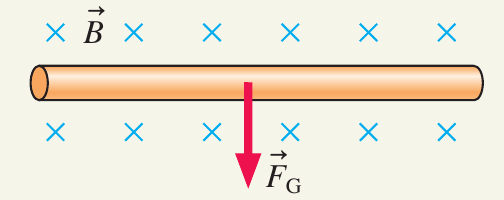
\includegraphics[width=0.55\linewidth]{figures/knight-fig29-44.png}
\end{center}
\figtask{Label $\vec B$'s direction, and sketch in the current
direction and $\vec F_B$ once you've worked out which way they go.}

\textbf{MODEL.} The wire floats if the magnetic force on it points
\bl[2.5cm] and has magnitude \bl[2.5cm], exactly balancing the
downward gravitational force.

\textbf{SOLVE --- set the forces equal.} With the wire perpendicular
to $\vec B$:

\[
F = IlB = \bl[5cm]
\]

The weight comes from the copper's density $\rho=8920\text{ kg/m}^3$
and the wire's volume. Write the mass as $m=\rho V$, with $V$ the
volume of a cylinder of radius $r$ and length $l$:

\[
IlB = \bl[7cm]
\]

\checkpoint{One factor appears on both sides of that equation and
cancels. Which one --- and why should the current needed to float the
wire \emph{not} depend on how long the wire is?}

Solve for the current:

\result[1.8cm]{$I = $}

Plug in $r=0.00050$ m, $g=9.80\text{ m/s}^2$, and the given $B$ and
$\rho$:

\eqline[0.2cm]{$I = $}

\textbf{Direction.} With $\vec B$ pointing into the page (as drawn),
the right-hand rule says the current must flow \bl[3cm] to make
$\vec F_B$ point \bl[2cm].

\checkpoint{The book notes this idea is only useful once you can get
current into and out of the floating segment. If the lead-in wires run
straight down to the segment (parallel to $\vec B$), why do \emph{they}
feel no force while the segment does?}

%============================================================
\nsec{Torque on a current loop}

Now put a whole square loop (side $l$, current $I$) in a uniform field
$\vec B$, with the loop's normal --- its magnetic moment $\vec m$ ---
at angle $\theta$ to $\vec B$. The field pushes on all four sides, but
two of those forces, $\vec F_{\text{front}}$ and $\vec F_{\text{back}}$,
are equal and opposite \emph{along the same line} and simply cancel.
The other two, $\vec F_{\text{top}}$ and $\vec F_{\text{bottom}}$, are
also equal and opposite --- so the \emph{net force} on the loop is
still zero --- but they act along \bl[4cm] lines, separated by a
moment arm $d$. A force pair like that doesn't translate the loop; it
\bl[2.5cm] it.

\begin{center}
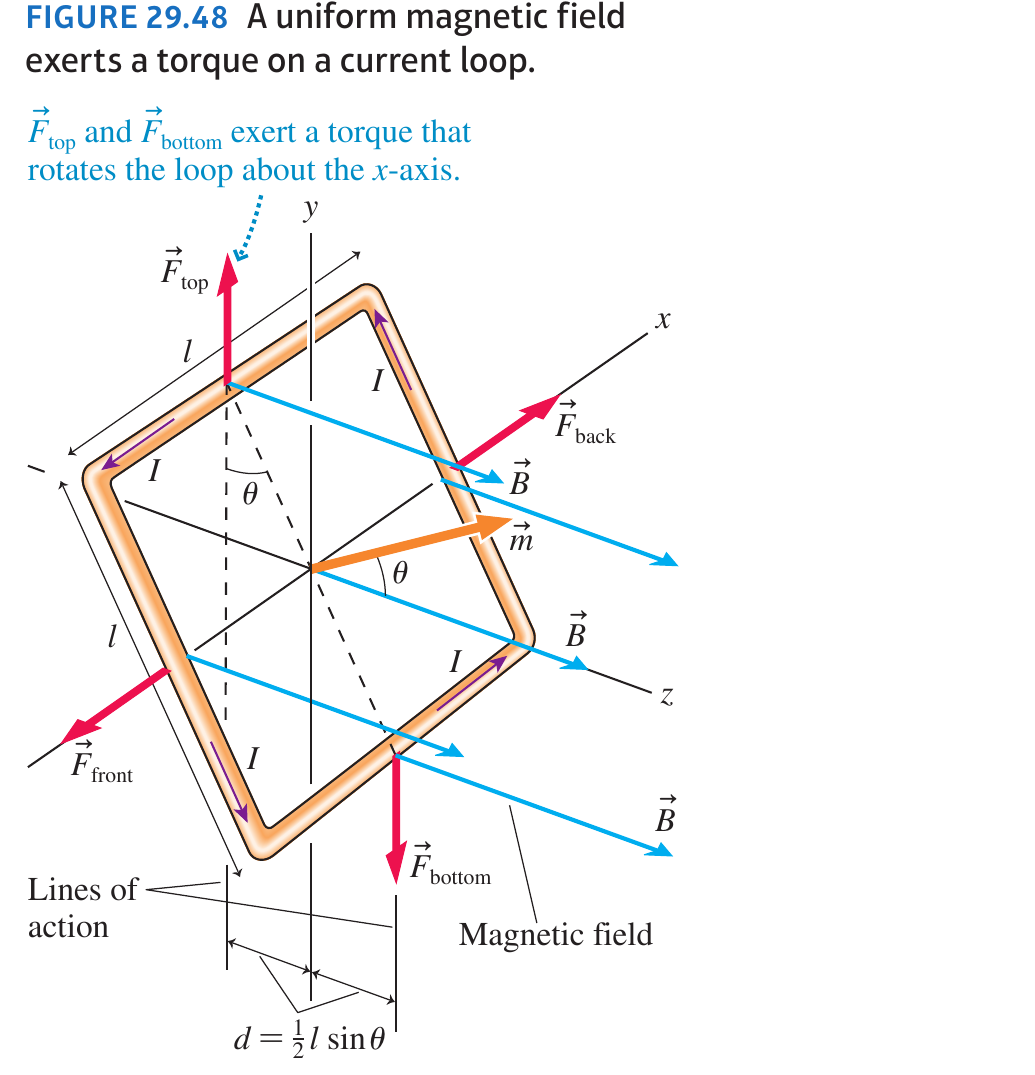
\includegraphics[width=0.62\linewidth]{figures/knight-fig29-48.png}
\end{center}
\figtask{Mark which pair of forces cancels outright, and which pair is
the one producing the torque.}

Each of $\vec F_{\text{top}}$, $\vec F_{\text{bottom}}$ has magnitude
$F=IlB$ (Section 1's result, with $\theta=90^\circ$ between the wire
and $\vec B$), and the moment arm for each is $d=\tfrac12 l\sin\theta$.
Torque is force times moment arm, and there are two force/arm pairs
acting together:

\[
\tau = 2Fd = 2(IlB)\left(\tfrac12 l\sin\theta\right) = \bl[5cm]
\]

The combination $Il^2=IA$ (area $A=l^2$ for this square loop) is the
loop's magnetic moment magnitude $m$ (or $m=NIA$ for $N$ turns instead
of just one). This result turns out to hold for a loop of \emph{any}
shape:

\result[1.8cm]{$\tau = $}

In vector form, since this is one more example of a cross product:

\eqline[0.2cm]{$\vec\tau = \bl[4cm]$}

\checkpoint{At what angle $\theta$ is this torque zero? At what angle
is it maximum? A compass needle is a magnetic dipole --- use your
answer to explain why a compass needle always ends up pointing along
$\vec B$, not across it.}

%============================================================
\nsec{Worked example: torque on a coil}

\textit{A flat coil has $N=40$ turns, each a square $l=3.0$ cm on a
side. The coil carries a current $I=1.5$ A and sits in a uniform field
$B=0.50$ T, with its magnetic moment at $\theta=35^\circ$ to the field
(as in Figure 29.48). What is the magnitude of the torque on the
coil?}

\textbf{MODEL.} The coil is a magnetic dipole with moment
$m=\bl[3cm]$; the torque follows directly from $\tau=mB\sin\theta$.

\textbf{SOLVE.} First find the area of one turn and the dipole moment:

\[
A = l^2 = \bl[5cm]
\]

\[
m = NIA = \bl[6cm]
\]

Now find the torque:

\result[1.8cm]{$\tau = mB\sin\theta = $}

Plug in the numbers:

\eqline[0.2cm]{$\tau = $}

\checkpoint{If you doubled the number of turns $N$ --- same loop size
$l$, same current $I$ --- would the torque go up, down, or stay the
same? What does that suggest about why real motors and galvanometers
wind \emph{many turns} of wire around the same coil, rather than using
a single loop?}

\end{document}
